\chapter{Конструкторский раздел}%
\label{cha:konstruktorskii_razdel}

\section{Последовательность действий для сокрытия присутствия пользователя}

На рисунке 2.1 показаны входные и выходные потоки данных и библиотека, необходимая для реализации поставленной задачи.

\begin{figure}[H]
    \centering
    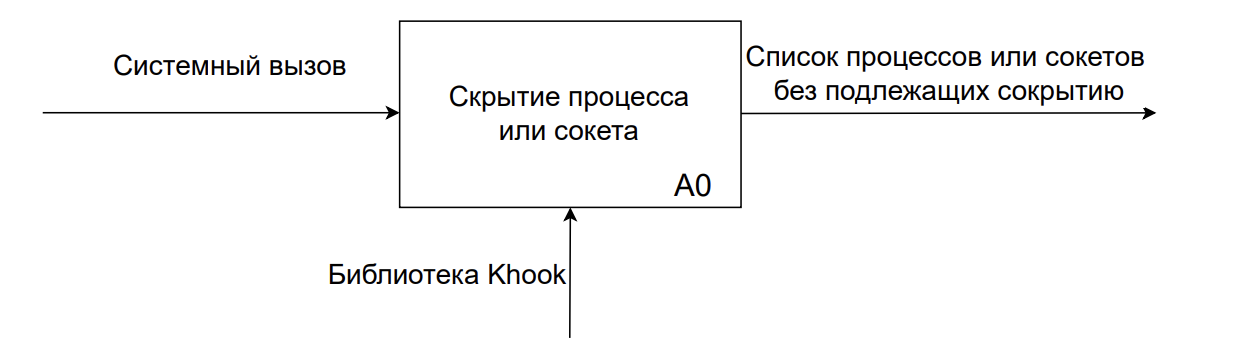
\includegraphics[scale=0.75]{pdf/1.png}
    \caption{IDEF0-диаграмма нулевого уровня}\label{img:net_hide_schemeeqq}
\end{figure}

Загружаемый модуль ядра должен выполнять последовательность действий, показанную на рисунке 2.2.

\begin{figure}[H]
    \centering
    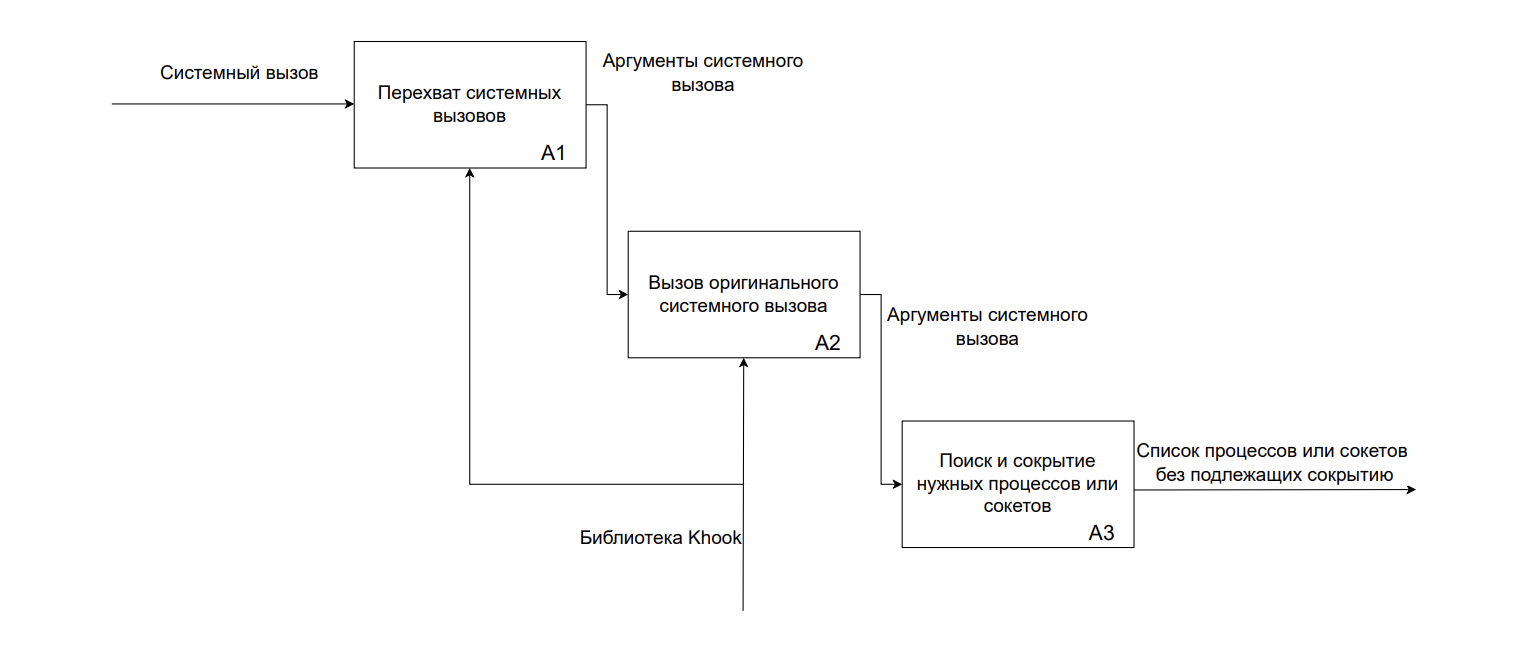
\includegraphics[scale=0.75]{pdf/2.png}
    \caption{IDEF0-диаграмма первого уровня}\label{img:net_hide_schemeeqq1}
\end{figure}


\section{Структура ПО}
На рисунке 2.3 приведена структура разрабатываемого программного обеспечения.

\begin{figure}[H]
    \centering
    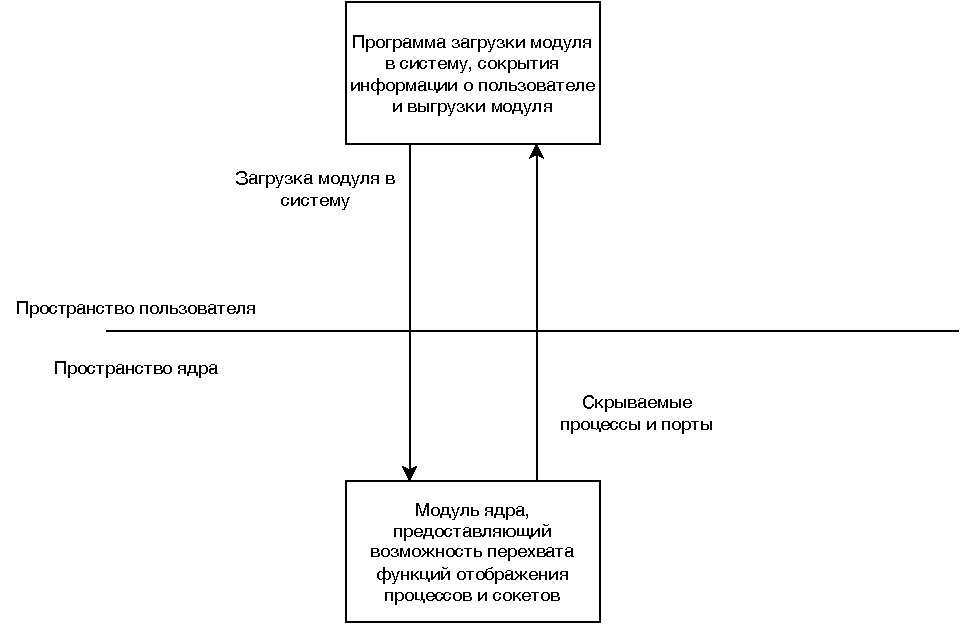
\includegraphics[scale=0.75]{pdf/struct.pdf}
    \caption{Структура ПО}\label{img:net_hide_schemee}
\end{figure}

\section{Сокрытие процессов}%
\label{sec:skrytie_protsessov}

Так как в ходе анализа с помощью утилиты strace было выявлено,
что для отображжения процессов используется системный вызов getdents,
в схеме алгоритма представлен наш обработчик этого вызова. В начале
алгоритма происходит вызов оригинального системного вызова, что показано
на рисунке 2.4.

\begin{figure}[H]
    \centering
    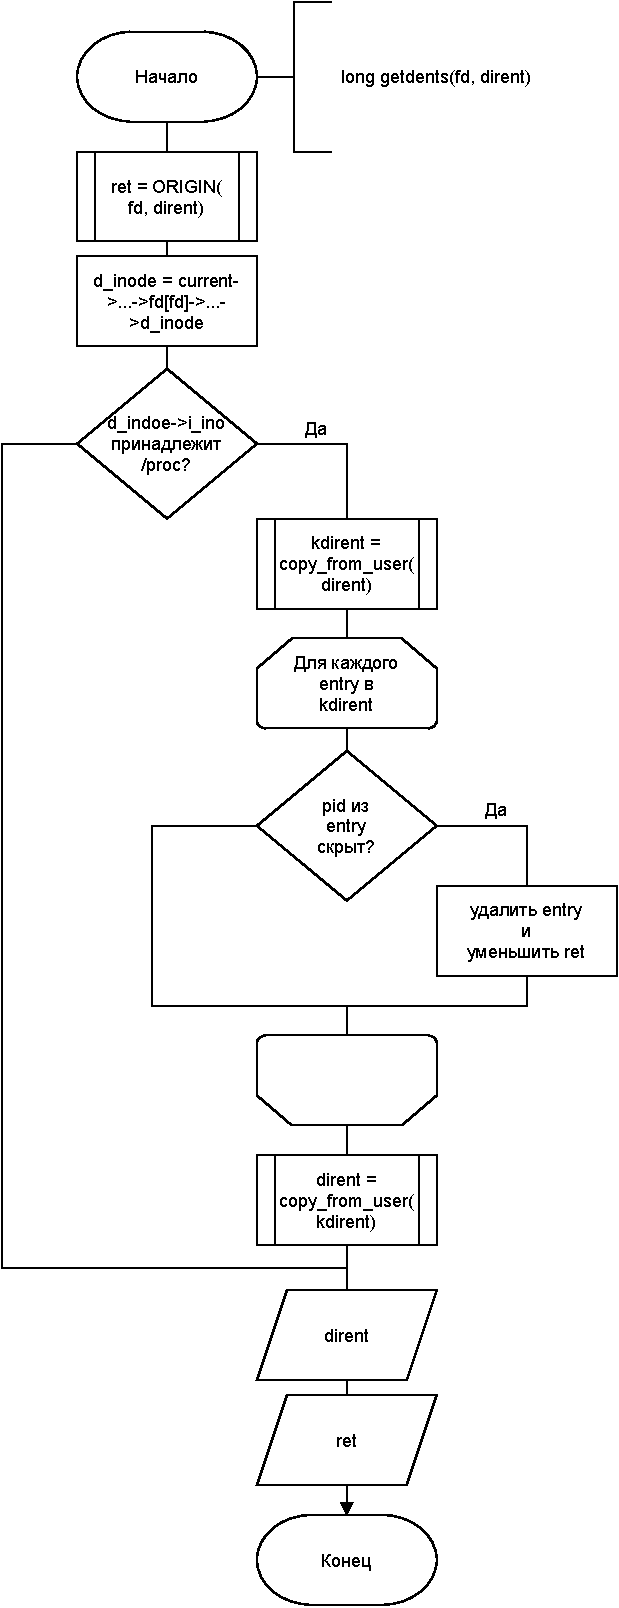
\includegraphics[scale=0.65]{pdf/oscw_proc.pdf}
    \caption{Алгоритм сокрытия процесса}\label{img:proc_hide_scheme}
\end{figure}

\section{Сокрытие сетевых сокетов}%
\label{sec:skrytie_setevykh_soketov}

Так как в ходе анализа с помощью утилиты strace было выявлено,
что для отображения сокетов используется, в том числе, системный вызов
tcp4\_seq\_show, в схеме алгоритма представлен наш обработчик этого вызова.

\begin{figure}[H]
    \centering
    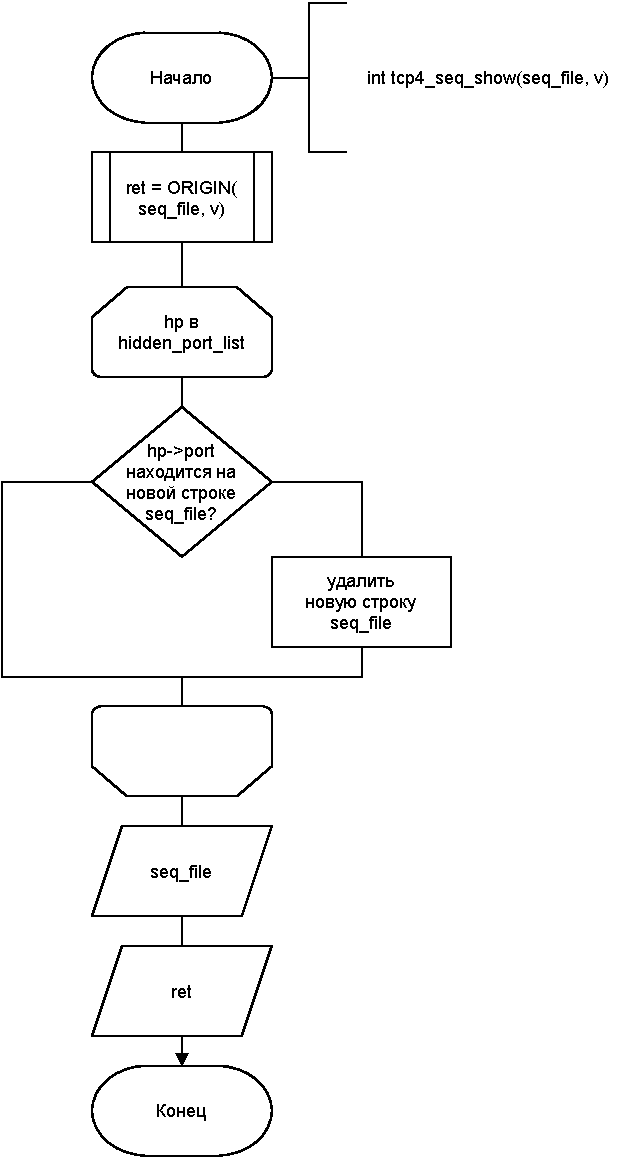
\includegraphics[scale=0.65]{pdf/oscw_net.pdf}
    \caption{Алгоритм сокрытия сетевых сокетов}\label{img:net_hide_scheme}
\end{figure}




\section{Выводы}%
\label{sec:vyvody}

В данном разделе была рассмотрена структура программного обеспечения.